\documentclass[UTF8]{ctexart}
\usepackage{bookmark}
\usepackage{geometry}
\usepackage{hyperref}
\geometry{a4paper,scale=0.8}
\usepackage{ctex}
\usepackage[style=caspervector,backend=biber,utf8]{biblatex}
\usepackage{booktabs}
\usepackage{array}
\usepackage{fancyhdr}
\pagestyle{fancy}
\fancyhf{}
\renewcommand\footrulewidth{1pt}
\lhead{王铠泽}
\rhead{PB18020766}
\chead{\href{mailto:volar@mail.ustc.edu.cn}{volar@mail.ustc.edu.cn}}
\rfoot{中国科学技术大学}
\lfoot{\today}
\usepackage{graphicx}
\usepackage{float}
\usepackage{subfigure}


\begin{document}

	\centering\textbf{\LARGE{计算物理A第七次作业}}
	
	
	王铠泽\qquad PB18020766
	
		
	\section{作业题目}
	
	\begin{itemize}
		\item 对一个实验谱数值曲线$  p(x) $ ,自设$  F(x) $,分别用直接抽样和舍选法
		对$p(x)$抽样。比较原曲线和抽样得到的曲线以验证。讨论抽样效率
			\begin{figure}[H]
			\centering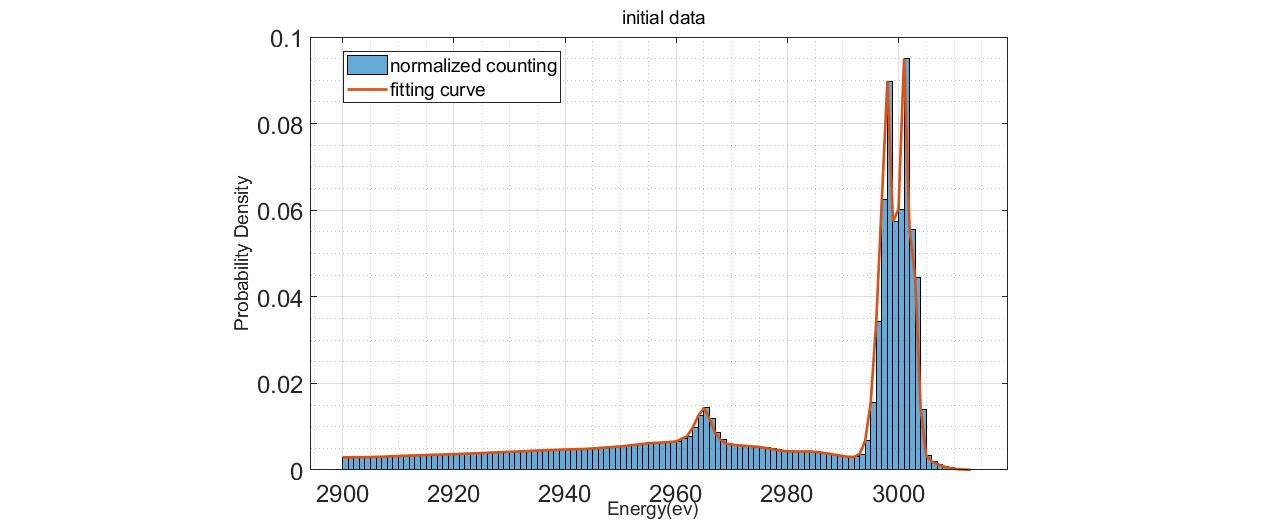
\includegraphics[width=6in]{../figure/curve}
			\caption{数据直方图}
			\end{figure}
	\end{itemize}
	
	\section{实现方法}
	
	\begin{itemize}
		\item 直接抽样
		
		本实验中直接抽样采用离散化的分布模型(若要得到连续性分布可以将$p(x)$进行线性插值得到相应的累计函数$P(X)$,再通过二分法求逆)。$p(k)=\frac{N_k}{\sum N_k}$
		
		设$\xi$为[0,1]上均匀抽样。若满足$P(k-1)<\xi\leq P(k)$,则取$E=k$作为抽样。
		
		其中$P(k)=\sum_{i=2899}^{k}p(k)$,$P(2899)=0,P(3013)=1$。
		\item 舍选法抽样
		
		采用分段式的阶梯函数作为$F(x)$。
		$$\left\{
		\begin{array}{lc}
			0.0143& 2900\leq x<2994\\
			0.0950& 2994\leq x < 3005\\
			0.0033& 3005\leq x\leq 3013
		\end{array}
		\right.$$
		示意图如下:
		\begin{figure}[H]
			\centering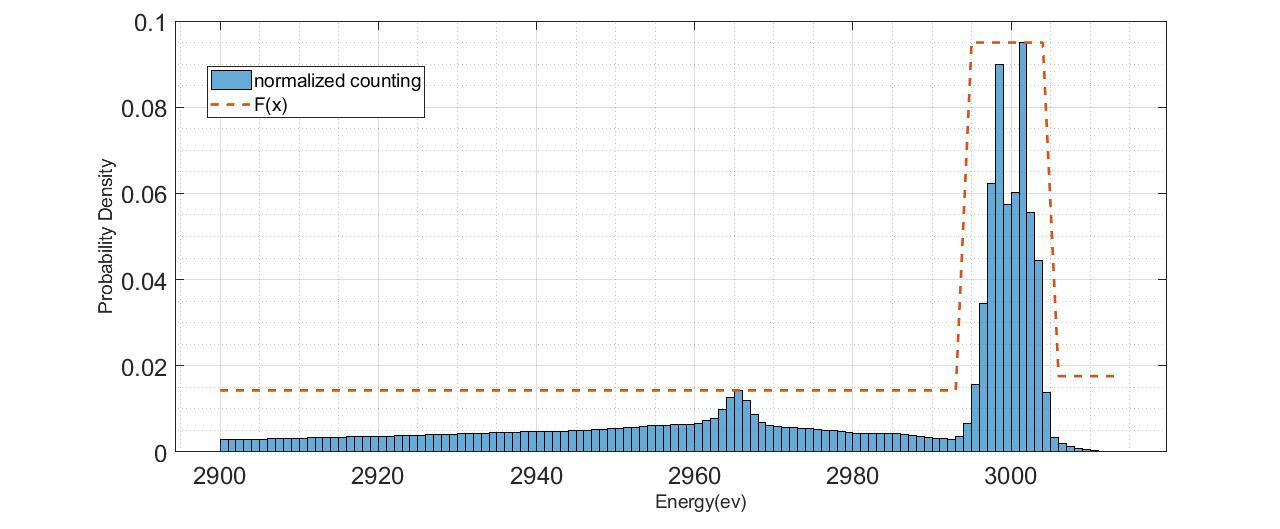
\includegraphics[width=6in]{../figure/curve2}
			\caption{阶跃型$F(x)$}
		\end{figure}
	
	其效率为$I=\frac{1}{\int_{2900}^{3013}F(x)dx}\approx0.413976$。$F(x)$归一化对应的累计函数为:
	
	$$H(x)=\left\{
	\begin{array}{lc}
	0.00591986x-17.1676& 2900\leq x<2994\\
	 0.0393277 x-117.191 & 2994\leq x < 3005\\
    0.00136612 x-3.11612 & 3005\leq x\leq 3013
	\end{array}
	\right.$$
	
	抽样方法:
	生成两个$[0,1]$上随机序列$\xi_1
	,\xi_2$。在$x$方向上,按$F(x)$分布抽样:$$\xi_x=H^{-1}(\xi_1)=\left\{
	\begin{array}{ll}
    168.923\xi_1+2900.00& 0\leq \xi_1<0.556466\\
	25.4274\xi_1+2979.86 & 0.556466\leq \xi_1 <0.988799\\
	732.00\xi_1+2281.00 & 0.988799\leq \xi_1 \leq 1\\
	\end{array}
	\right.$$
	在$y$方向上,按$\frac{1}{F(\xi_x)}$的均匀分布抽样:$$\xi_y=F(\xi_x)\xi_2$$
	比较关系:
	$$\left\{
	\begin{array}{lc}
	\xi_y<p(\xi_x)& accept\\
	\xi_y\geq p(\xi_x)& reject\\
	\end{array}
	\right.
	$$
	在最后一步比较大小时,我们采用了线性插值的办法:对于$floor(\xi_x)\leq\xi_x\leq ceil(\xi_x)$,估计值为:
	$$p(\xi_x)=p[floor(\xi_x)]\cdot\frac{\xi_x-ceil(\xi_x)}{floor(\xi_x)-ceil(\xi_x)}+p[ceil(\xi_x)]\cdot\frac{\xi_x-floor(\xi_x)}{ceil(\xi_x)-floor(\xi_x)}$$
	其中$floor,ceil$分别为向下,向上取整函数。
	\end{itemize}
	
	\section{程式说明}
	\begin{itemize}
		\item sampling.c
		
		该程式包含两大部分:1.使用直接抽样法抽取曲线对应数据;2.采用舍选抽样法抽取曲线对应数据。
	
		包含以下函数:
		
		\subitem double F (double x)
		
		这个函数就是前述的$F(x)$。
		
		\item rdm.h
			
		这是一个包含了使用16807产生器生成指定长度的$[0,1]$上均匀分布随机数函数的头文件。
		
		\subitem void rdm(int N,double *x,int method)
		
		该函数将输入的指针$x$对应的长度为$N$的数组用$[0,1]$上的随机数填满。method是关于初始种子的选择。method=0:默认种子;method=1,时间种子。程式中故意采用$sleep$函数就是为了得到不同的时间种子。
		
		\item time\_seed.txt
		
		16807产生器抽样时对应的时间种子数据(1个种子)和对应抽样方法(后者是手动加入)。
		
		\item direct\_sampling/reject\_sampling.txt
		
		记录了生成的随机数数据文件。
	\end{itemize}
	
	\section{计算结果}
	
	在总点数为$10000$的条件下得到如下分布直方图。其中红色曲线是依据原始数据拟合而得。
	
	
	\begin{figure}[H]
		\centering  %图片全局居中
		\subfigure[直接抽样]{
			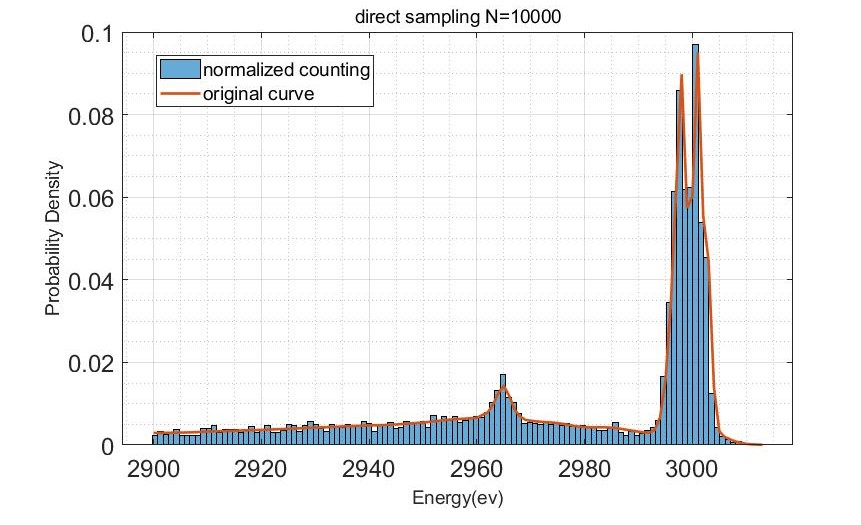
\includegraphics[width=0.6\textwidth]{../figure/direct.jpg}}
		\subfigure[舍选抽样,$\eta=0.4210$]{
			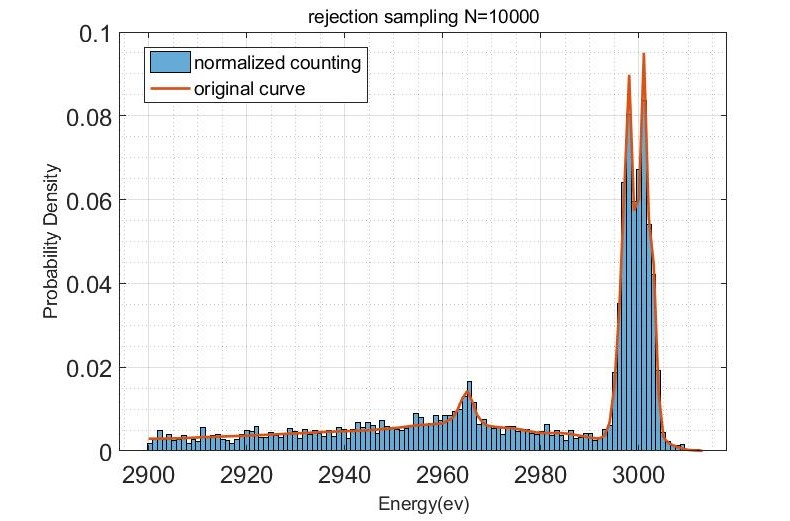
\includegraphics[width=0.6\textwidth]{../figure/reject.jpg}}
		\caption{$N=10000$时归一化直方图分布}
	\end{figure}
%	
	\begin{figure}[H]
		\centering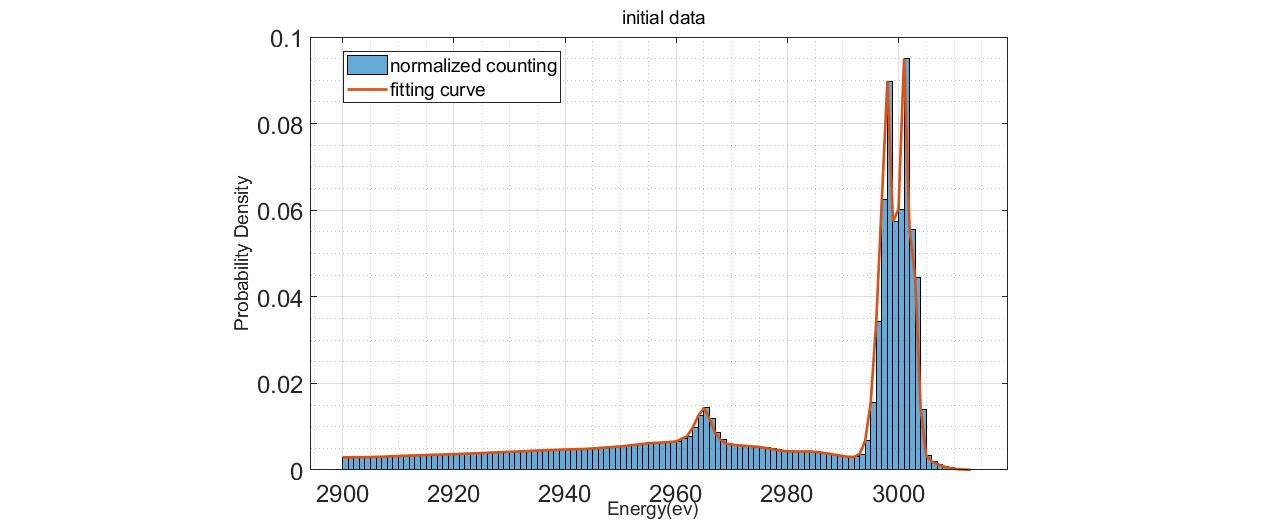
\includegraphics[width=6in]{../figure/curve}
		\caption{原图}
	\end{figure}
	\textbf{\begin{flushleft}
			可见两者都和实验曲线有良好拟合。
	\end{flushleft}}
	
%		\begin{figure}[H]
%			\centering  %图片全局居中
%			\subfigure[$N=10000$,$\eta=0.793200$]{
%				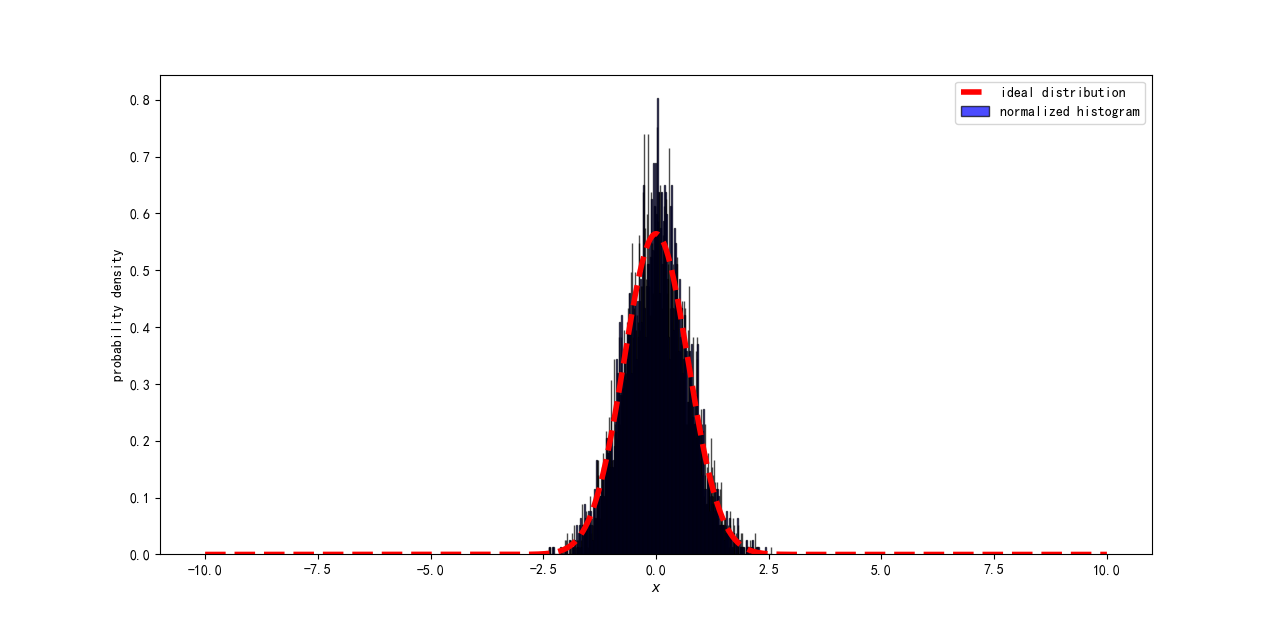
\includegraphics[width=0.6\textwidth]{../figure/N=10000.png}}
%			\subfigure[$N=100000$,$\eta=0.798740$]{
%				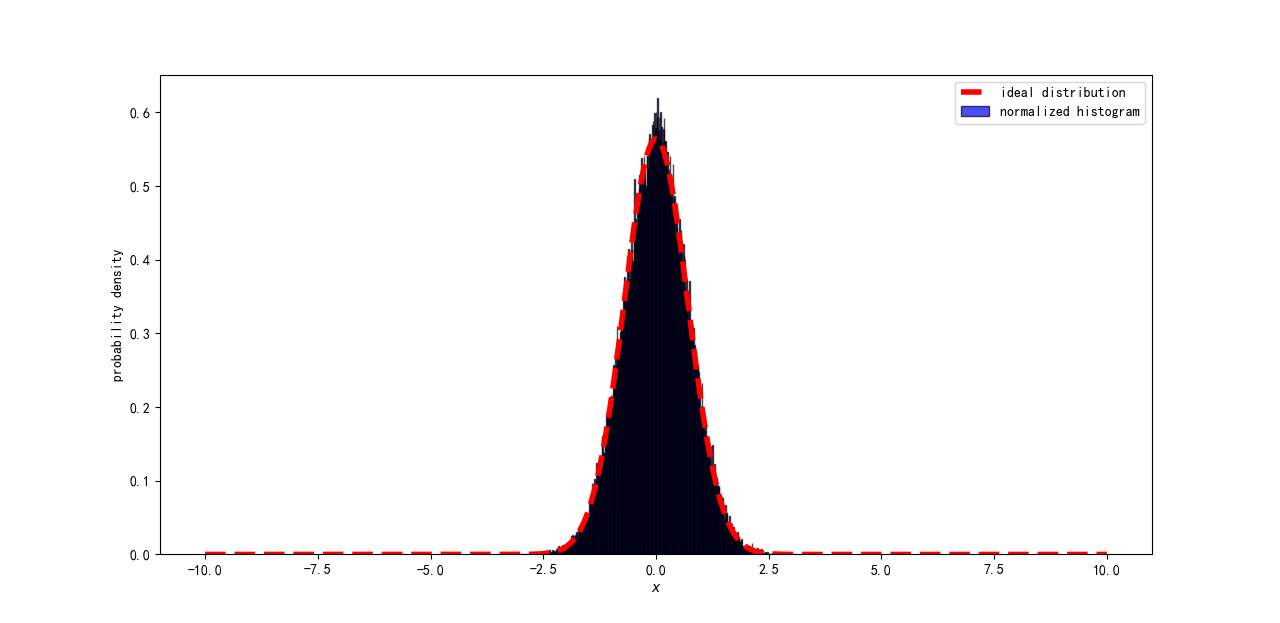
\includegraphics[width=0.6\textwidth]{../figure/N=100000.png}}
%			\subfigure[$N=1000000$,$\eta=0.798477$]{
%				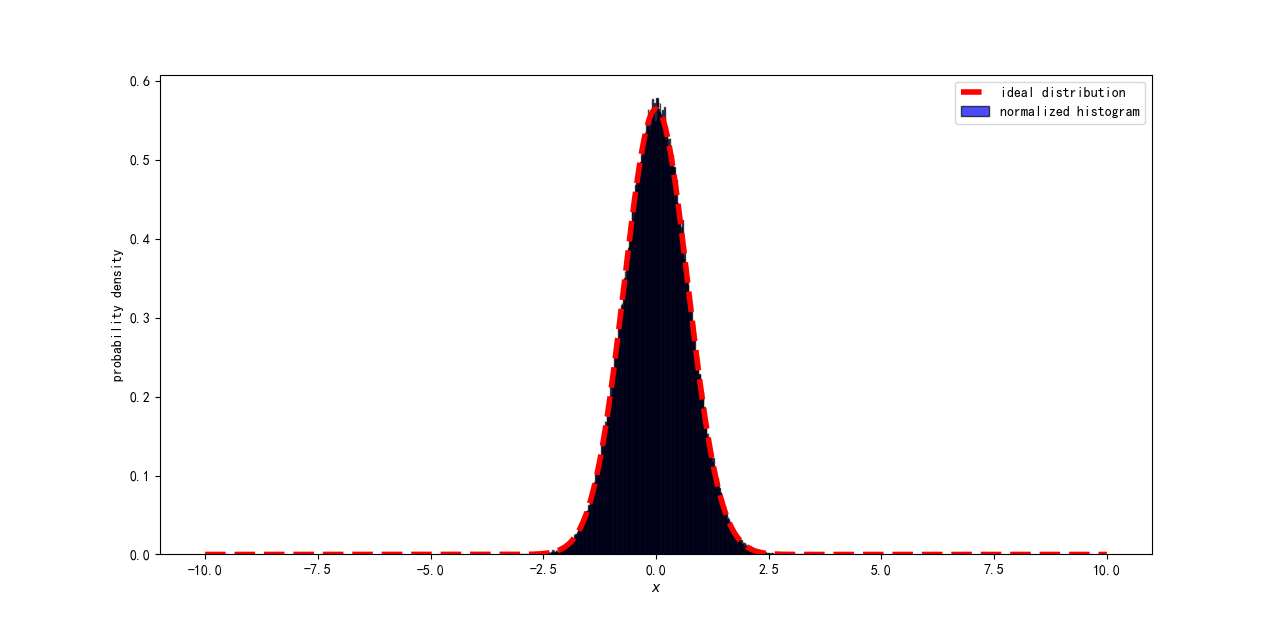
\includegraphics[width=0.6\textwidth]{../figure/N=1000000.png}}
%			\caption{归一化直方图}
%		\end{figure}

	\section{总结}
	\begin{itemize}
		\item 本次实验分别采用直接抽样法和舍选抽样法对实验数据曲线进行抽样。两种抽样的效果差不多,舍选抽样在$3000ev$左右峰处拟合更为理想,其原因可能是在舍选法中做了线性插值而直接抽样是直接视为离散分布。在峰处变化剧烈,采用线性插值能减小误差。
		\item 直接抽样法的抽样效率为$\%100$,而舍选抽样在本实验中约为$40\%$,明显偏低。为了提高抽样效率,可能更加精细的分出更多的阶梯。但这样做实在是大大增加了在代码层面的工作量,总效率也不见得提升。
		\item 实际应用中,应该根据数据的个数,数据分布情况,要求精度等来进行抽样方法选择。
	\end{itemize}
	\clearpage
\end{document}